% Chapter Template

\chapter{Introduction} % Main chapter title

% Importance
% Motivation
% Application
% challenges
% thises Content
% 3Pages of intro 
% RelatedW0Rk  



\label{chp:intro} % Change X to a consecutive number; for referencing this chapter elsewhere, use \ref{ChapterX}
\section{Coronavirus Disease}

COronaVIrus Disease 2019 (COVID-19) is a severe respiratory tract infection that can range from mild to lethal \cite{acter2020evolution}. COVID-19 is a contagious disease that can readily spread through direct or indirect contact with an infected person \cite{singhal2020review}. COVID-19 is caused by severe acute respiratory syndrome coronavirus 2 (SARS-CoV-2). COVID-19 initially appeared in Wuhan, China late 2019 and spread worldwide \cite{hui2020continuing}. World Health Organization (WHO) declared the outbreak of COVID-19 as a Public Health Emergency of International Concern in January 2020, and a pandemic in March 2020 \cite{platto2020covid19}.
Ongoing SARS-CoV-2 infections have not only devastated human lives but also significantly damaged the financial health of both developing and developed countries. Therefore, there is an urgent need to control the pandemic by accelerating the development and mass production of efficacious vaccines against SARS-CoV-2. Healthcare practitioners, researchers, and policymakers around the globe were thrown a challenge to deliver adequate prevention and treatment modalities to combat the pandemic. From the initial stage of this pandemic, scientists were focused on either repurposing the existing drugs or developing vaccines against COVID-19 \cite{le2020evolution}. Figure \ref{NorCovCXR} illustrates the difference between the COVID-19 and normal lungs.

Typical diagnostic tools for COVID-19 are virus’ nucleic acid by real-time reverse transcription polymerase chain reaction (rRT-PCR), transcription-mediated amplification (TMA), or reverse transcription loop-mediated isothermal amplification (RT-LAMP) from a nasopharyngeal swab \cite{tahamtan2020real}.  These manual traditional methods are time-consuming and complex. Chest X-rays (CXR) and chest CT offer fast screening methods for COVID-19 \cite{salehi2020coronavirus}\cite{wu2020new}\cite{zu2020coronavirus}. CXR and chest CT are preferred when RT-PCR testing is not available in time \cite{erickson1993advanced}. CXR has many advantages over chest CT including the widespread of acquisition devices, low cost, and the speed of the acquisition\cite{narin2021automatic}\cite{brenner2007computed}\cite{rubin2020role}\cite{shi2020review}. These advantages lead CXR to be a fixed routine for hindering COVID-19 spread. 

\begin{figure}%
    \centering
    \begin{subfigure}[b]{0.4\textwidth}
        \centering
        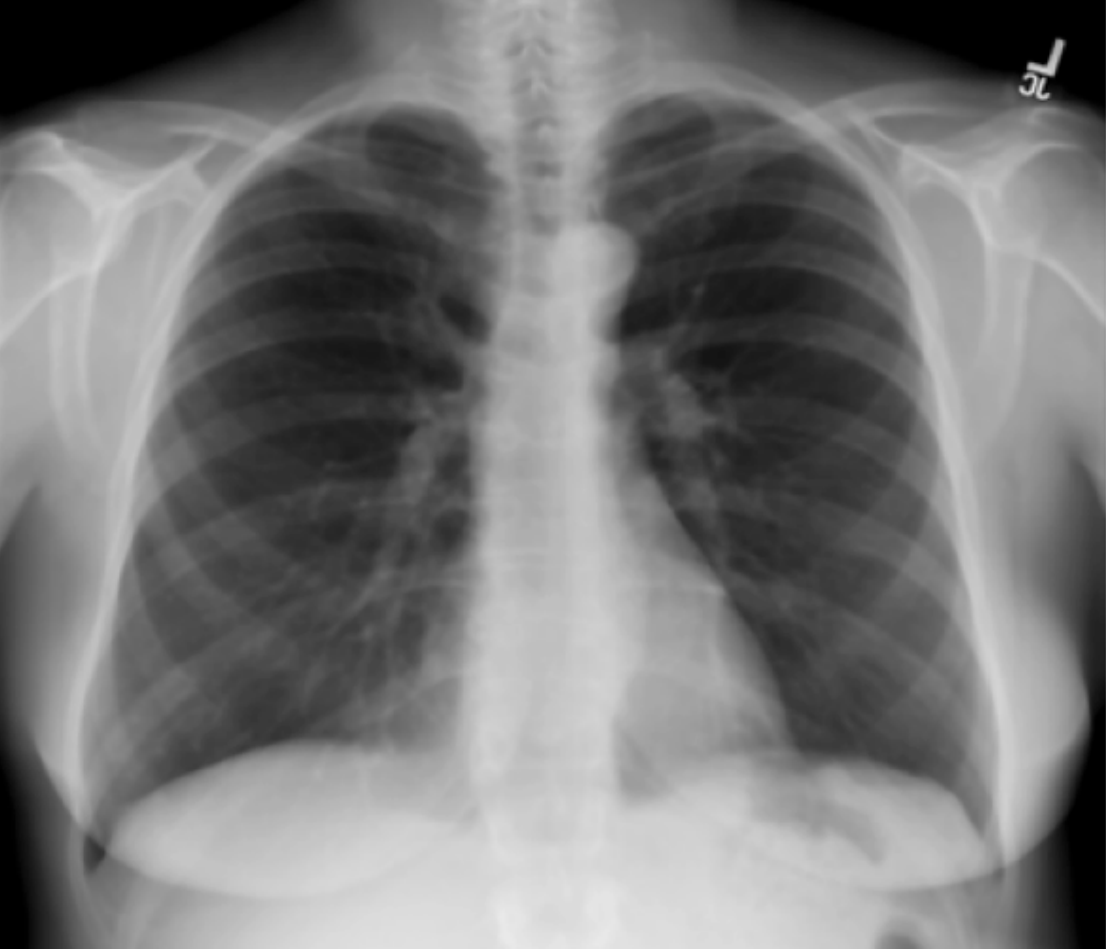
\includegraphics[width=\textwidth]{Figures/introNormCXR.png}
        \caption{Chest X-ray image of normal lung.}
        \label{NorCXR}
    \end{subfigure}
    % \hfill
     \begin{subfigure}[b]{0.4\textwidth}
         \centering
         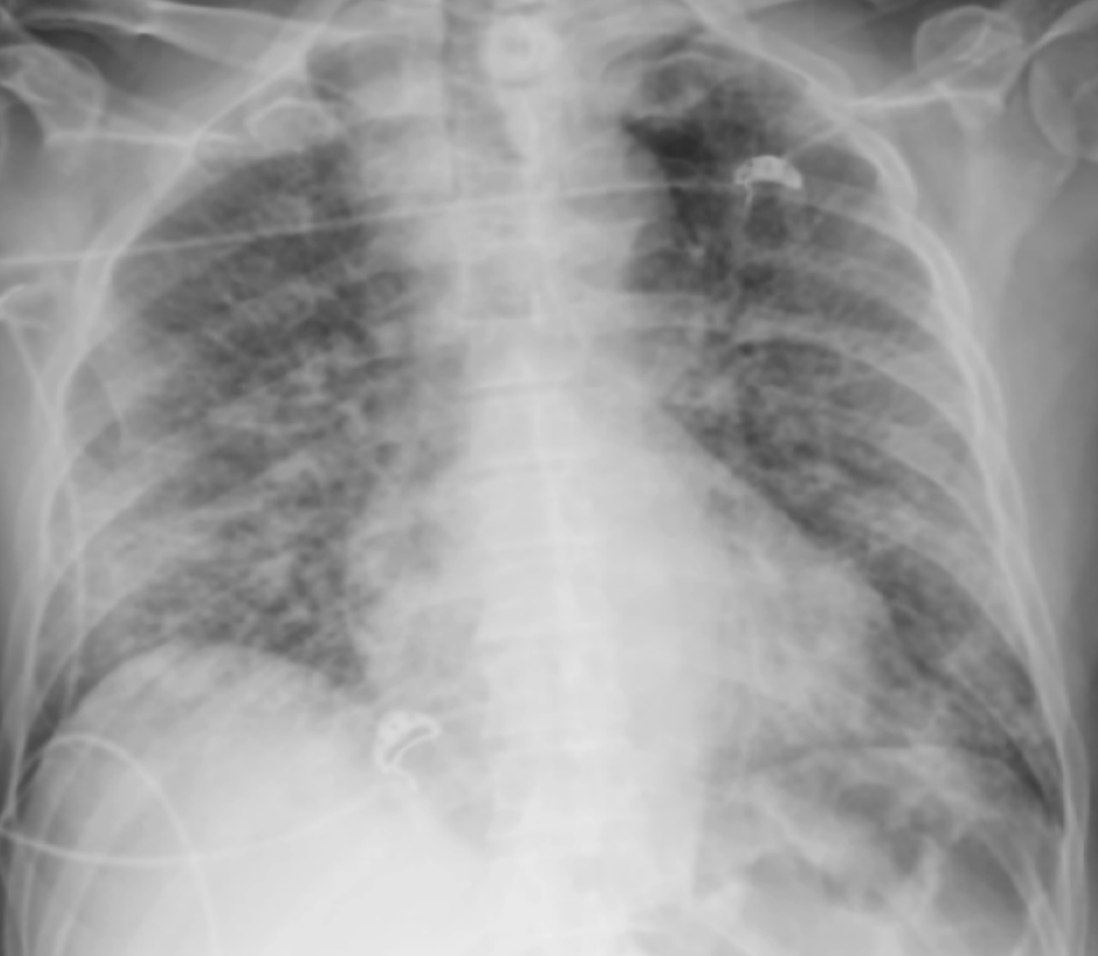
\includegraphics[width=\textwidth]{Figures/intoCovidCXR.png}
         \caption{Chest X-Ray image of COVID-19 patient}
         \label{CovCXR}
     \end{subfigure}
    \caption{Samples of CXR images of Normal and COVID-19 pneumonia}%
    \label{NorCovCXR}%
\end{figure}
\section{Research Problem Statement} 
The rapid spread of COVID-19 caused by SARS-CoV-2 has not only resulted in significant loss of life but has also strained the financial systems of both developing and developed countries. This widespread transmission places immense pressure on healthcare systems, emphasizing the urgent need for efficient diagnostic methods. While CNNs have shown promise in various computer vision tasks, they have limitations such as scalability and computational cost.
This thesis tackles the following problems of the COVID-19 classification.
\begin{itemize}
    \item High classification accuracy for COVID-19 detection.
    \item Proposing a model with lower computational requirements.
\end{itemize} 
 This thesis aims to address these challenges by proposing two CNN architectures for COVID-19 diagnosis: one focusing on lightweight design and the other on multiscale feature extraction. The primary problem addressed in this research is to develop effective and efficient CNN models for COVID-19 diagnosis that can provide high accuracy while minimizing computational complexity and overfitting. These models are evaluated using the QaTa-Cov19 benchmark dataset, aiming to achieve superior performance with significantly fewer trainable parameters compared to existing methods in the literature.

\section{Motivation}
Figure \ref{hospitalRoutine} illustrates a typical Egyptian hospital routine for reducing COVID-19 spread among healthcare workers. This process is performed for every visitor to the hospital. Phases of CBC tests and PCR tests are automated and do not consume time. While CXR image diagnosing involves human factors that act as a bottleneck of the process. This process can be fully automated using image classification models. As a consequence \textit{1)} Total time required for every visitor will be reduced. \textit{2)} The load of radiologists is reduced. 

\begin{figure}%
    \centering
        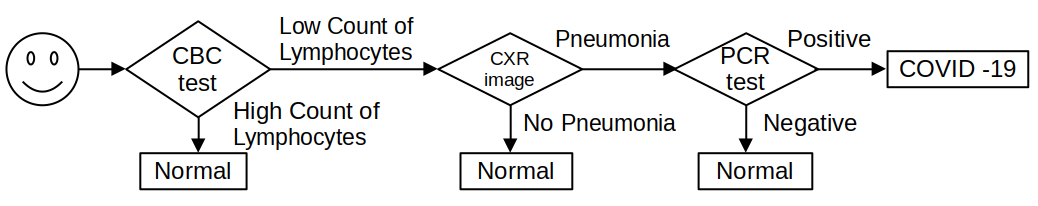
\includegraphics[width=\textwidth]{Figures/HosPitalCovidRoutine.png}
        \caption{Typical hospitals routine of reducing COVID-19 spread}
        \label{hospitalRoutine}
\end{figure}

Deep learning \cite{lecun2015deep} models, namely convolutional Neural Network (CNN) \cite{lecun1989handwritten}, have shown a great performance in computer vision problems such as object detection \cite{erhan2014scalable}\cite{girshick2014rich}\cite{sermanet2013overfeat}\cite{redmon2016you} and object recognition \cite{simonyan2014very}\cite{he2016deep}. CNN is initially introduced in \cite{lecun1989handwritten}. CNN  is based on hierarchical learning of the convolutional kernels which are organized in layers \cite{krizhevsky2012imagenet}. The function of lower-order layers is to learn low-level features such as edges and corner points \cite{zeiler2014visualizing}. Higher order layers learn high-level features such as objects \cite{zeiler2014visualizing}. Typical CNN architecture is several convolutional layers that are connected sequentially \cite{simonyan2014very}. This sequential connection of the layers does not scale well for deep CNN \cite{he2016deep}. CNN shows great performance when it has a large number of layers \cite{he2016deep}. To allow CNN to take advantage of the deep architecture, residual connections are used \cite{he2016deep}. Residual connections solve the vanishing gradient problem when gradients approach zeros. Also, residual connections allow the reuse of earlier features \cite{huang2017densely}. Layers with residual connections are easier to optimize than plain layers as they can easily approximate the identity mapping \cite{he2016deep}. In this thesis, CNN is used to automate and accelerate the diagnosing pipeline of COVID-19.


\begin{figure}%
    \centering
        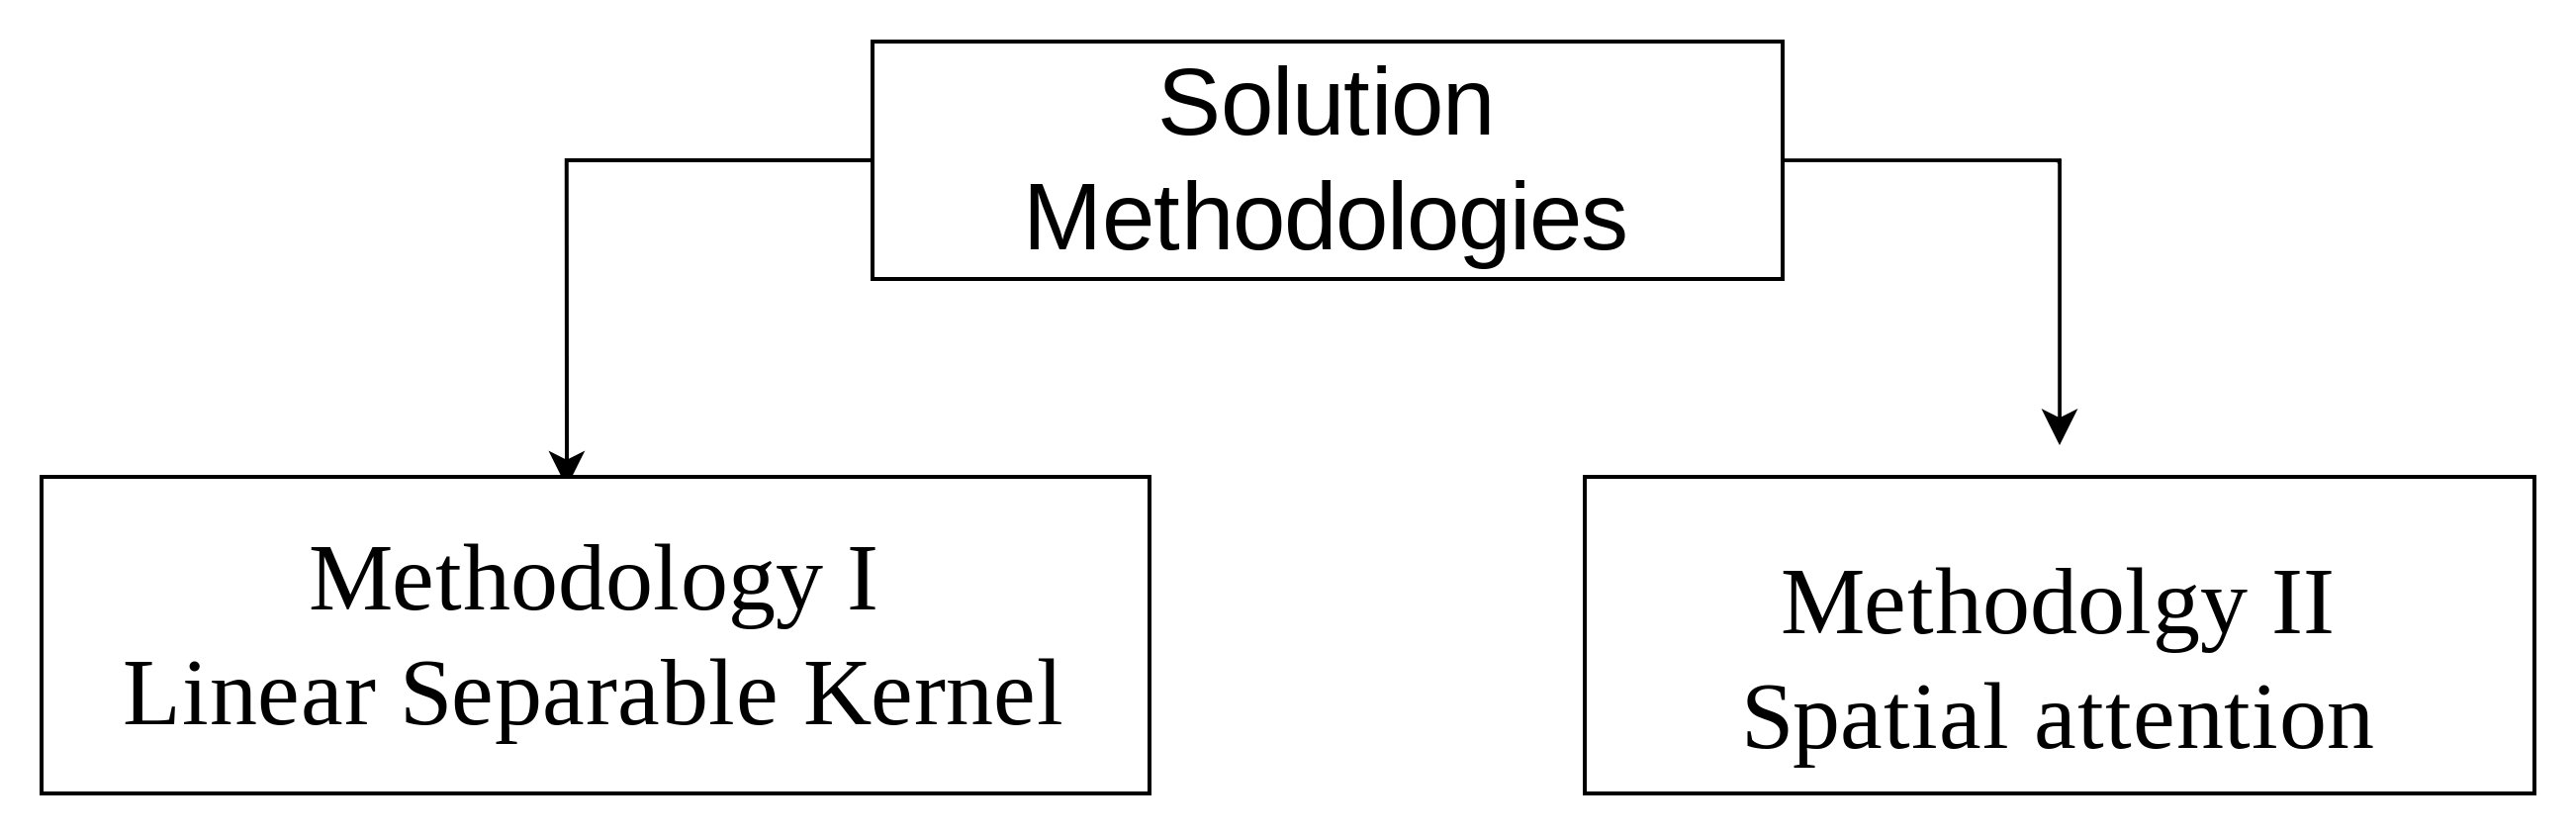
\includegraphics[width=\textwidth]{Figures/SolutionMethodologies.png}
        \caption{Solution Methodologies proposed in this thesis}
        \label{solMeth}
\end{figure}


\section{Detection Challenges}
Like many computer vision problems, COVID-19 has the following challenges
\begin{itemize}

\item \textbf{Availability of Data.} CNN is a deep learning technique that requires a large number of training Images. However, the current COVID-19 dataset are small-size dataset which is challenging to train large networks with. 
\item \textbf{Scale.} Like many computer vision models CNN is a scale variant. CNN can not recognize images with scales different from the scales it trained on.
\item \textbf{Vanishing Gradient Problem.} Deep CNN suffers a vanishing gradient which prevents CNN parameters from being updated.
\item \textbf{Exploding Gradient Problem.} Deep CNN suffers Exploding gradient which makes CNN diverge.
\end{itemize}
Proposed Systems try to overcome these problems as will be detailed in chapters \ref{chp:proposed1}.

\section{Thesis Objective and Contributions}
The objective of this thesis is to improve classification accuracy and reduce the computational complexity of detecting COVID-19 cases from CXR Images. Contributions of this thesis are as follows.
\begin{itemize}
    \item \textit{Lightweight classification model.} A Lightweight classification model with a very low parameter number is proposed for the classification of the CXR images. It reduces the computational complexity which allows deployment on mobile devices and saves bandwidth of the network during the model distribution process. 
    \item \textit{Scale invariant model.}  Pneumonia scales in CXR are not uniformly distributed which prevents CNN from recognizing infrequent scales. Scale-invariant model is proposed for the detection of COVID-19 pneumonia at different scales.
    \item \textit{High Detection accuracy.} Proposed systems provide superior performance according to various classification metrics.
\end{itemize}

\section{Thesis Organization}
This thesis is organized as follows: 
\begin{itemize}
    \item \textbf{Chapter \ref{chp:background}}: includes required Background to understand the Thesis.Also includes and illustrates the recent and related work in the COVID-19 detection literature. 
    \item \textbf{Chapter \ref{chp:proposed1}}: presents the proposed work I which presents a lightweight classification model. Also presents the proposed work II which includes the scale-invariant model for COVID-19 classification. 
    \item \textbf{Chapter \ref{chp:results}}: illustrates the experimental results for both proposed work I and II and quantitative analysis of the proposed work I and II is provided.
    \item \textbf{Chapter \ref{chp:concl}}: concludes the thesis and provides planning for the future work as an extension of the proposed approach
\end{itemize}